\section[I Sistemi]{I Sistemi}
\sectionframe{images/covers/cover_intro.jpg}{Intro}

\subsection[Intro]{Intro}

% Pastorello: intro_statistical_learning
% https://www.javatpoint.com/machine-learning
\begin{frame}
	\frametitle{Sistema e Stato}
	
	\begin{block}{Sistema}
		Un \textbf{sistema} è un insieme di elementi in relazione tra di loro secondo leggi ben precise che concorrono al raggiungimento di un obiettivo comune.
	\end{block}
	\begin{block}{Stato}
		Il sistema, in base al dati ricevuti in ingresso ed alla sua natura, evolve istante dopo istante in una nuova situazione che è chiamata \textbf{stato}.
	\end{block}
\end{frame}


\begin{frame}
	\frametitle{Esempi di sistemi e stati}
	
	\begin{block}{Esempi di sistemi e stati}
		Potremmo paragonare lo stato di un sistema ad una fotografia del sistema in un dato istante:
		\begin{itemize}
			\item \textbf{Sistema contatore del gas}: in tale contesto lo \textbf{stato} del sistema corrisponde alla cifra dei Smc (standard metro cubo) consumati fino a quell'istante.
			\item \textbf{Sistema distributore automatico delle bibite}: in tale contesto lo \textbf{stato} del sistema corrisponde alle bibite presenti nei vari slot ed al denaro per restituire il resto presente nella macchina.
		\end{itemize}
	\end{block}
\end{frame}


\begin{frame}
	\frametitle{Catalogazione dei sistemi}
	
	\begin{block}{È possibile catalogare i sistemi in tre grandi categorie:}
		\begin{itemize}
			\item \textbf{Sistemi naturali}: \textit{sono i sistemi esistenti in natura} .\\
			Si cita come esempio il sistema solare. Anche per il corpo umano si utilizza il termine sistema inteso come insieme di componenti che, aggregati in modo opportuno, svolgono specifiche funzioni; si hanno per esempio il sistema digerente e il sistema circolatorio.
			\item \textbf{Sistemi artificiali}: \textit{sono i sistemi creati dall'uomo}.\\
			Esempi di sistemi artificiali sono il sistema computer, un distributore di bibite, un'ascensore oppure il sistema di regolazione della temperatura dell'acqua di una piscina.
			\item \textbf{Sistemi misti}: \textit{sono sistemi naturali sui quali l’uomo è intervenuto}.\\
			Si cita come esempio il caso di un sistema destinato alla produzione di energia elettrica che viene realizzato deviando un corso d'acqua.
		\end{itemize}
	\end{block}
\end{frame}


\begin{frame}
	\frametitle{Un qualunque sistema X}
	
	\begin{block}{Potremmo rappresentare qualunque sistema X nel seguente modo:}
		\begin{itemize}
			\item Riceve un insieme di informazioni di partenza \textbf{I} che chiameremo \textbf{inputs}.
			\item Può modificare lo/gli stato/stati \textbf{S} nel quale si può trovare in un determinato istante.
			\item Fornisce un insieme di risposte \textbf{O} che chiameremo \textbf{outputs}.
		\end{itemize}
		
		\begin{figure}[!htbp]
			\centering
			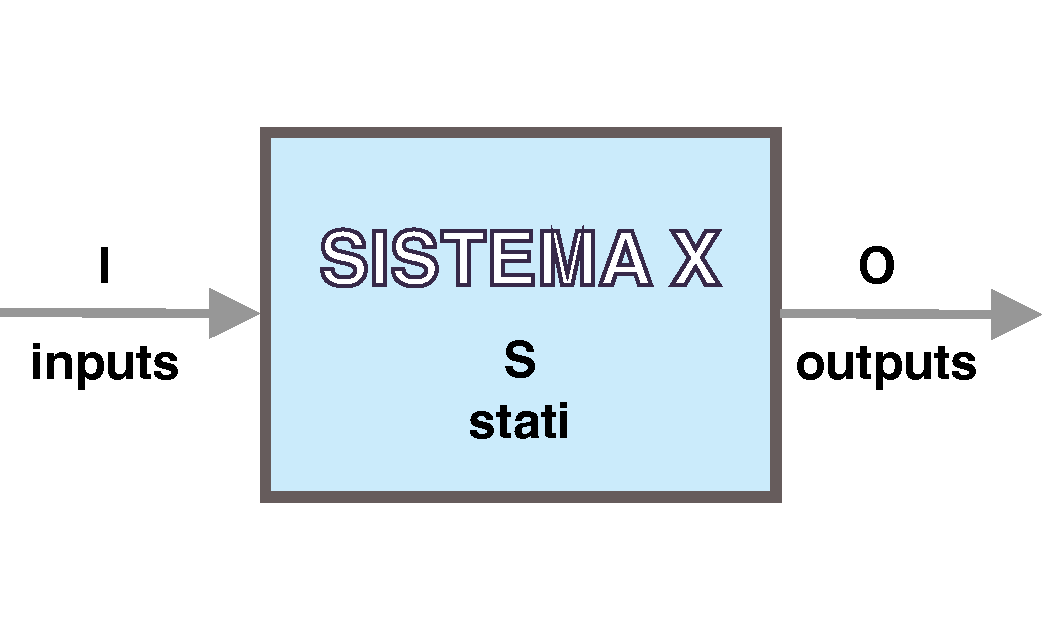
\includegraphics[width=0.55\linewidth]{images/1_i_sistemi/sistemaX.pdf}
					%\caption{}
		\end{figure}
		\vspace{0.4em}
	\end{block}
\end{frame}


\begin{frame}
	\frametitle{Un qualunque sistema X}
	
	\begin{block}{Le grandezze che determinano un sistema:}
		Un sistema è basato su quattro grandezze principali\\
		(in generale indicheremo in maiuscolo l’insieme di tutte le variabili e in minuscolo la singola variabile):\vspace{1em}
		\begin{itemize}
			\item Ingressi ($\pmb{I}$): formati dal set delle variabili di ingresso ($\pmb{i_1}$, $\pmb{i_2}$, ..., $\pmb{i_n}$)
			\item Uscite ($\pmb{O}$): formate dal set delle variabili di uscita ($\pmb{o_1}$, $\pmb{o_2}$, ..., $\pmb{o_n}$)
			\item Stati ($\pmb{S}$): formati dal set delle variabili di stato ($\pmb{s_1}$, $\pmb{s_2}$, ..., $\pmb{s_n}$)
			\item Tempo ($\pmb{T}$): formati dalle variabili tempo ($\pmb{t_1}$, $\pmb{t_2}$, ..., $\pmb{t_n}$)\\nelle quali si studia il sistema
		\end{itemize}
	\end{block}
\end{frame}


\begin{frame}
	\frametitle{Un qualunque sistema X}
	
	\begin{block}{Le grandezze che determinano un sistema:}
		\vspace{1.5em}
		\begin{figure}[!htbp]
			\centering
			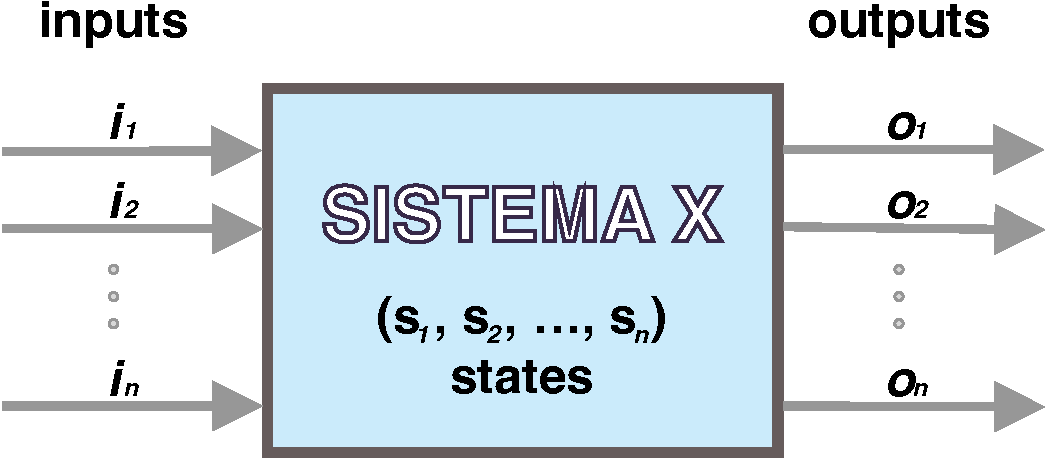
\includegraphics[width=0.65\linewidth]{images/1_i_sistemi/sistemaX2.pdf}
					%\caption{}
		\end{figure}
		\vspace{1.5em}
	\end{block}
\end{frame}



\begin{frame}
	\frametitle{Un esempio di sistema:}
	
%	\begin{block}{}
		\begin{itemize}
			\item \textbf{Set degli input}:
				\begin{itemize}
					\item[--] le monete inserite ($i_1$ = coins).
					\item[--] la scelta/selezione fatta sul distributore ($i_2$ = choice).
				\end{itemize}
			\item \textbf{Set degli stati}:
				\begin{itemize}
					\item[--] le monete all'interno del distributore ($s_1$ = coins).
					\item[--] le bibite presenti all'interno del distributore ($s_2$ = drinks).
				\end{itemize}
			\item \textbf{Set degli output}:
				\begin{itemize}
					\item[--] la bibita in uscita ($o_1$ = drink).
					\item[--] il resto ($s_2$ = change).
				\end{itemize}
		\end{itemize}
		\vspace{1.5em}
		\begin{figure}[!htbp]
			\centering
			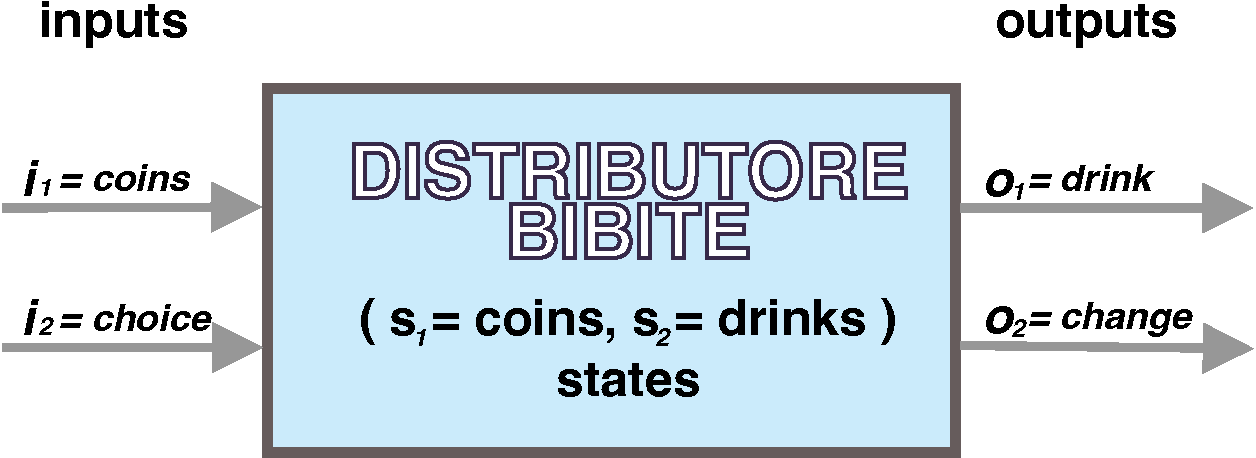
\includegraphics[width=0.60\linewidth]{images/1_i_sistemi/sistemaX3.pdf}
					%\caption{}
		\end{figure}
		\vspace{1.5em}
%	\end{block}
\end{frame}

